\section{Escrevendo um gramática}

\begin{frame}[fragile]{Expressões regulares vs. gramáticas livres de contexto}

    \begin{itemize}
        \item Qualquer construção que pode ser descrita por uma expressão regular pode ser descrita por uma gramática
        \pause

        \item A recíproca nem sempre é verdadeira
        \pause

        \item Por exemplo, a expressão regular $(a\ |\ b)^*abb$ e a gramática
        \[
            \begin{array}{l}
                A_0\to aA_0\ |\ bA_0\ |\ aA_1 \\
                A_1\to bA_2 \\
                A_2\to bA_3 \\
                A_3\to \code{apl}{∊}
            \end{array}
        \]
        descrevem a mesma linguagem
        \pause

        \item É possível converter automaticamente um autômatico finito não-determinístico em uma gramática que gere a mesma linguagem do AFN
    \end{itemize}

\end{frame}

\begin{frame}[fragile]{Algoritmo de conversão de um AFN para uma gramática livre de contexto}

    \begin{algorithmic}[1]
        \Require{um AFN}
        \Ensure{uma gramática livre de contexto} 

        \For{cada estado $i$ do AFN}
            \State{crie um símbolo não-terminal $A_i$ da gramática}
            \If{o estado $i$ possui um transição para o estado $j$ com rótulo $a$}
                \State{introduza a produção $A_i\to aA_j$ na gramática}
            \ElsIf{o estado $i$ possui um transição para o estado $j$ com rótulo \code{apl}{∊}}
                \State{introduza a produção $A_i\to A_j$ na gramática}
            \EndIf
            \If{o estado $i$ é um estado de aceitação}
                \State{introduza a produção $A_i\to \code{apl}{∊}$ na gramática}
            \ElsIf{o estado $i$ é o estado de partida}
                \State{torne o estado $A_i$ o símbolo de partida da gramática}
            \EndIf
        \EndFor
    \end{algorithmic}

\end{frame}

\begin{frame}[fragile]{Razões para o uso de expressões regulares para definir a estrutura léxica}

    \begin{enumerate}
        \item As regras léxicas de uma linguagem geralmente são simples, sendo as expressões regulares suficientes para descrevê-las
        \pause

        \item As expressões regulares, em geral, descrevem os tokens da linguagem de forma mais concisa e clara do que as gramáticas livres de contexto
        \pause

        \item É possível gerar analisadores léxicos mais eficientes a partir de expressões regulares do que a partir de gramáticas arbitrárias
        \pause

        \item A separação da estrutura léxica da estrutura sintática permite a modularização da interface de vanguarda
    \end{enumerate}

\end{frame}

\begin{frame}[fragile]{Verificando a linguagem gerada por uma gramática}

    \begin{itemize}
        \item A prova que uma gramática $G$ gera uma linguagem $L(G)$ é feita em duas etapas:
        \pause
        \begin{enumerate}
            \item mostrar que cada cadeia gerada por $G$ está em $L(G)$
            \pause

            \item mostrar que cada cadeia em $L(G)$ pode ser gerada por $G$
        \end{enumerate}
        \pause

        \item Por exemplo, considere a gramática
        \[
            S\to (S)S\ |\ \code{apl}{∊}
        \]
        \pause

        \item Esta gramática gera todas as cadeias de parêntesis balanceadas
        \pause

        \item Para provar esta afirmação, primeiro é preciso provar que qualquer cada sentença derivável de $S$ é balanceada
        \pause

        \item Esta prova é feita por indução no número de passos da derivação
    \end{itemize}

\end{frame}

\begin{frame}[fragile]{Verificando a linguagem gerada por uma gramática}

    \begin{itemize}
        \item Em apenas um passo de derivação, a única cadeia gerada é a cadeia vazia \code{apl}{∊}, a qual é trivialmente balanceada
        \pause

        \item Suponha que qualquer derivação com menos do que $n$ passos gere uma cadeia balanceada
        \pause

        \item Uma derivação com exatamente $n$ passos tem a forma
        \[
            S\Rightarrow (S)S \overset{\scalebox{0.5}*}{\Rightarrow} (x)S \overset{\scalebox{0.5}*}{\Rightarrow} (x)y
        \]
        onde $x$ e $y$ são derivações com que $n$ passos
        \pause

        \item Pela hipótese de indução, $x$ e $y$ são balanceadas e, portanto, a derivação $S$ com exatamente $n$ passos também é balanceada
    \end{itemize}

\end{frame}

\begin{frame}[fragile]{Verificando a linguagem gerada por uma gramática}

    \begin{itemize}
        \item A prova que qualquer cadeia balanceada é derivável a partir de $S$ é feita por meio de indução no comprimento da cadeia
        \pause

        \item A menor cadeia balanceada é a cadeia vazia, que é derivável a partir de $S$ por meio da produção $S\to \code{apl}{∊}$
        \pause

        \item Suponha que todas as cadeias balanceadas com comprimento menor do que $2n$ sejam deriváveis a partir de $S$ e que $w$ seja uma cadeia balanceada de tamanho
            $2n$
        \pause

        \item Certamente $w$ inicia com um parêntesis à esquerda
        \pause

        \item Seja $(x)$ o menor prefixo de $w$ com o mesmo número de parêntesis à esquerda e à direita
        \pause

        \item Assim, $w = (x)y$, onde $x$ e $y$ são cadeias balanceadas com comprimento menor do que $2n$
        \pause

        \item Pela hipótese de indução, $x$ e $y$ são deriváveis a partir de $S$
        \pause

        \item Assim, $w$ é derivável a partir de $S$, por meio da derivação
        \[
            S\Rightarrow (S)S \overset{\scalebox{0.5}*}{\Rightarrow} (x)S \overset{\scalebox{0.5}*}{\Rightarrow} (x)y
        \]
    \end{itemize}

\end{frame}

\begin{frame}[fragile]{Eliminando a ambiguidade}

    \begin{itemize}
        \item Uma gramática pode ser reescrita para eliminar possíveis ambiguidades
        \pause

        \item Por exemplo, considere a gramática abaixo, que torna o \code{apl}{else} opcional:
        \[
            \begin{array}{rcl}
                cmd & \to & \textbf{if}\ expr\ \textbf{then}\ cmd \\
                & | & \textbf{if}\ expr\ \textbf{then}\ \textbf{else}\ cmd \\
                & | & \textbf{outro}
            \end{array}
        \]
        \pause

        \item Na gramática, \textbf{outro} significa qualquer outro enunciado
        \pause

        \item Esta gramática é ambígua: a cadeia
        \[
            \textbf{if}\ E_1\ \textbf{then if}\ E_2\ \textbf{then}\ S_1\ \textbf{else}\ S_2
        \]
        possui duas árvores gramaticais distintas
    \end{itemize}

\end{frame}

\begin{frame}[fragile]{Primeira árvore gramatical para a expressão `$\textbf{if}\ E_1\ \textbf{then if}\ E_2\ \textbf{then}\ S_1\ \textbf{else}\ S_2$'}

    \begin{figure}
        \centering

        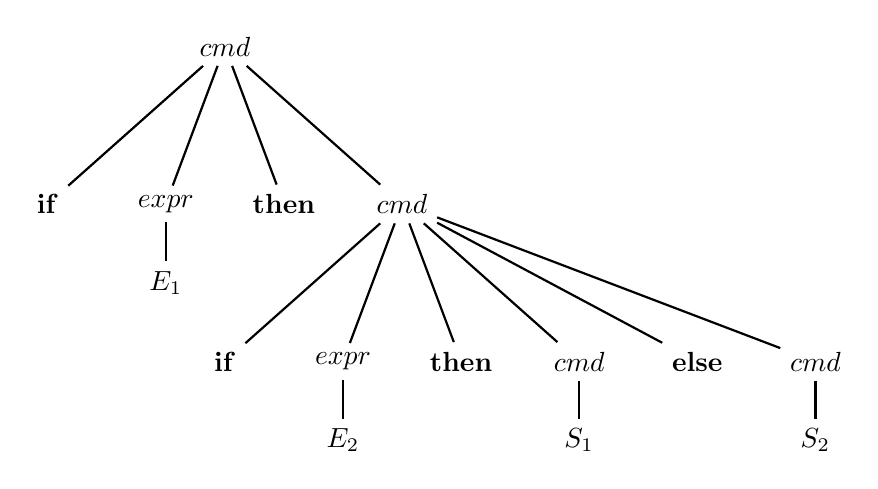
\begin{tikzpicture} 
            \node (A) at (2.25, 6) { $cmd$ };

            \node (B1) at (0, 4) { \textbf{if} };
            \node (B2) at (1.5, 4) { $expr$ };
            \node (B3) at (3, 4) { \textbf{then} };
            \node (B4) at (4.5, 4) { $cmd$ };

            \node (C0) at (1.5, 3) { $E_1$ };
            \node (C1) at (2.25, 2) { \textbf{if} };
            \node (C2) at (3.75, 2) { $expr$ };
            \node (C3) at (5.25, 2) { \textbf{then} };
            \node (C4) at (6.75, 2) { $cmd$ };
            \node (C5) at (8.25, 2) { \textbf{else} };
            \node (C6) at (9.75, 2) { $cmd$ };

            \node (D1) at (3.75, 1) { $E_2$ };
            \node (D2) at (6.75, 1) { $S_1$ };
            \node (D3) at (9.75, 1) { $S_2$ };

            \draw[thick] (A) to (B1);
            \draw[thick] (A) to (B2);
            \draw[thick] (A) to (B3);
            \draw[thick] (A) to (B4);
            \draw[thick] (B2) to (C0);
            \draw[thick] (B4) to (C1);
            \draw[thick] (B4) to (C2);
            \draw[thick] (B4) to (C3);
            \draw[thick] (B4) to (C4);
            \draw[thick] (B4) to (C5);
            \draw[thick] (B4) to (C6);

            \draw[thick] (C2) to (D1);
            \draw[thick] (C4) to (D2);
            \draw[thick] (C6) to (D3);
        \end{tikzpicture} 
    \end{figure}

\end{frame}

\begin{frame}[fragile]{Segunda árvore gramatical para a expressão `$\textbf{if}\ E_1\ \textbf{then if}\ E_2\ \textbf{then}\ S_1\ \textbf{else}\ S_2$'}

    \begin{figure}
        \centering

        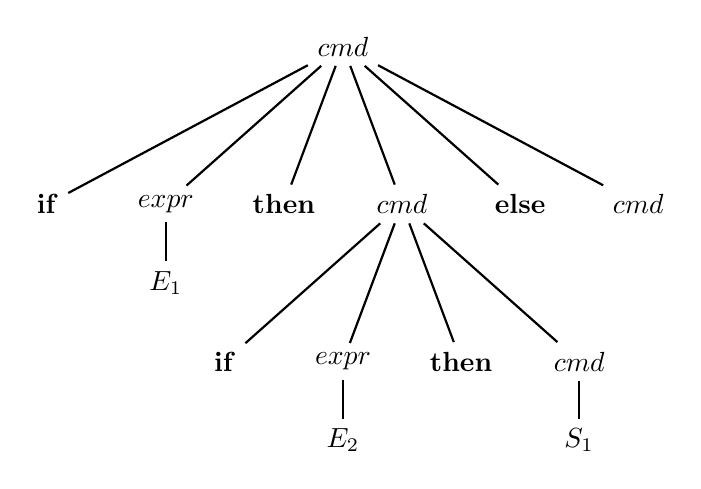
\begin{tikzpicture} 
            \node (A) at (3.75, 6) { $cmd$ };

            \node (B1) at (0, 4) { \textbf{if} };
            \node (B2) at (1.5, 4) { $expr$ };
            \node (B3) at (3, 4) { \textbf{then} };
            \node (B4) at (4.5, 4) { $cmd$ };
            \node (B5) at (6, 4) { \textbf{else} };
            \node (B6) at (7.5, 4) { $cmd$ };

            \node (C0) at (1.5, 3) { $E_1$ };
            \node (C1) at (2.25, 2) { \textbf{if} };
            \node (C2) at (3.75, 2) { $expr$ };
            \node (C3) at (5.25, 2) { \textbf{then} };
            \node (C4) at (6.75, 2) { $cmd$ };

            \node (D1) at (3.75, 1) { $E_2$ };
            \node (D2) at (6.75, 1) { $S_1$ };

            \draw[thick] (A) to (B1);
            \draw[thick] (A) to (B2);
            \draw[thick] (A) to (B3);
            \draw[thick] (A) to (B4);
            \draw[thick] (A) to (B5);
            \draw[thick] (A) to (B6);
            \draw[thick] (B2) to (C0);
            \draw[thick] (B4) to (C1);
            \draw[thick] (B4) to (C2);
            \draw[thick] (B4) to (C3);
            \draw[thick] (B4) to (C4);

            \draw[thick] (C2) to (D1);
            \draw[thick] (C4) to (D2);
        \end{tikzpicture} 
    \end{figure}

\end{frame}

\begin{frame}[fragile]{Reescrita para a eliminação da ambiguidade}

    \begin{itemize}
        \item Na maioria das linguagens, a primeira das duas árvores seria a esperada
        \pause

        \item A regra geral é associar cada \textbf{else} ao \textbf{then} anterior mais próximo ainda não associado
        \pause

        \item Para reescrita, a ideia é que um enunciado entre um \textbf{then} e um \textbf{else} precisa estar associado, isto é, não pode terminar em um
            \textbf{then} não associado a um \textbf{else}
        \pause
    \end{itemize}

    \[
        \begin{array}{rcl}
            cmd & \to & cmd\_associado \\
                & | & cmd\_nao\_associado \\
            cmd\_associado & \to & \textbf{if}\ expr\ \textbf{then}\ cmd\_associado\ \textbf{else}\ cmd\_associado \\
            & | & \textbf{outro} \\
            cmd\_nao\_associado & \to & \textbf{if}\ expr\ \textbf{then}\ cmd \\
            & | & \textbf{if}\ expr\ \textbf{then}\ cmd\_associado\ \textbf{else}\ cmd\_nao\_associado
        \end{array}
    \]
\end{frame}
